% Nguồn SGK Toán 9 Tập hai — Bài tập cuối chương X, trang 108--110:
% https://cdn3.olm.vn/upload/thuvienso/4491669493-page-108-1771844570596.png
% https://cdn3.olm.vn/upload/thuvienso/4491669493-page-109-1771844570926.png
% https://cdn3.olm.vn/upload/thuvienso/4491669493-page-110-1771844571273.png
%
% Nguồn SBT Toán 9 Tập hai — Ôn tập chương X, PDF page 69--71:
% SBT TOÁN 9 TẬP 2.pdf
% SHA-256: 5ff01fd213d1adc75f9c54b4408d6a9642a4d8038e685040efef3311a196196c
% PDF page 69 là trang chồng ranh giới: phần trên còn Bài 32 (10.13),
% phần dưới mới bắt đầu Ôn tập chương X. Không lấy phần 10.13 vào đây.
% Không lấy nội dung từ LỜI GIẢI -- HƯỚNG DẪN -- ĐÁP SỐ.

\section*{Bài tập cuối chương X}

\begin{exercises}
    \subsection{Bài tập cuối chương X}

    \textbf{A. TRẮC NGHIỆM}

    \begin{questions}[resume=SGK]
        \item Khi quay hình chữ nhật $ABCD$ một vòng quanh cạnh $AB$ ta được một hình trụ có bán kính đáy bằng độ dài đoạn thẳng
        \begin{tasks}(4)
            \task $AB$.
            \task $CD$.
            \task $AD$.
            \task $AC$.
        \end{tasks}
        \par\noindent\answerbox\par

        \item Cho tam giác $ABC$ vuông tại $A$ có $AB=4$ cm, $BC=5$ cm. Khi quay tam giác $ABC$ một vòng quanh cạnh $AC$ ta được một hình nón có chiều cao bằng
        \begin{tasks}(4)
            \task $4$ cm.
            \task $3$ cm.
            \task $5$ cm.
            \task $9$ cm.
        \end{tasks}
        \par\noindent\answerbox\par

        \item Diện tích mặt cầu có đường kính $10$ cm là
        \begin{tasks}(4)
            \task $10\pi$ cm$^2$.
            \task $400\pi$ cm$^2$.
            \task $50\pi$ cm$^2$.
            \task $100\pi$ cm$^2$.
        \end{tasks}
        \par\noindent\answerbox\par

        \item Cho hình nón có bán kính đáy $R=2$ cm, độ dài đường sinh $l=5$ cm. Diện tích xung quanh của hình nón đã cho bằng
        \begin{tasks}(4)
            \task $\dfrac{10\pi}{3}$ cm$^2$.
            \task $\dfrac{50\pi}{3}$ cm$^2$.
            \task $20\pi$ cm$^2$.
            \task $10\pi$ cm$^2$.
        \end{tasks}
        \par\noindent\answerbox\par

        \item Một mặt phẳng đi qua tâm hình cầu, cắt hình cầu theo một hình tròn có diện tích $9\pi$ cm$^2$. Thể tích của hình cầu bằng
        \begin{tasks}(4)
            \task $972\pi$ cm$^3$.
            \task $36\pi$ cm$^3$.
            \task $6\pi$ cm$^3$.
            \task $81\pi$ cm$^3$.
        \end{tasks}
        \par\noindent\answerbox\par
    \end{questions}

    \textbf{B. TỰ LUẬN}

    \begin{questions}[resume=SGK]
        \item Cho hình trụ có bán kính đáy bằng $20$ cm, chiều cao bằng $30$ cm.
        \begin{questions}
            \item Tính diện tích xung quanh của hình trụ.
            \item Tính thể tích của hình trụ.
        \end{questions}
        \answerline
        \answerline

        \item Cho hình nón có bán kính đáy bằng $9$ cm, độ dài đường sinh bằng $15$ cm (H.10.34).

        \begin{center}
            \begin{tikzpicture}
                \coordinate (O) at (0,0);
                \coordinate (S) at (0,3);
                \coordinate (A) at (-1.7,0);
                \coordinate (B) at (1.7,0);
                \draw (A) arc[start angle=180,end angle=360,x radius=1.7,y radius=.45];
                \draw[dashed] (A) arc[start angle=180,end angle=0,x radius=1.7,y radius=.45];
                \draw (S)--(A) (S)--(B);
                \draw[dashed] (S)--(O);
                \draw (O)--(B);
                \pic[draw, angle radius=3mm] {right angle=S--O--B};
                \node[above=1pt of S] {$S$};
                \node[left=1pt of A] {$A$};
                \node[right=1pt of B] {$B$};
                \node[below=2pt of O] {$O$};
                \node[right=3pt] at ($(S)!0.55!(B)$) {$15$ cm};
                \node[above=2pt] at ($(O)!0.55!(B)$) {$9$ cm};
            \end{tikzpicture}

            \textit{Hình 10.34}
        \end{center}

        \begin{questions}
            \item Tính diện tích xung quanh của hình nón.
            \item Tính thể tích của hình nón.
            \item Diện tích toàn phần của hình nón bằng tổng diện tích xung quanh và diện tích đáy. Tính diện tích toàn phần của hình nón đã cho.
        \end{questions}
        \answerline
        \answerline
        \answerline

        \item Quả bóng rổ sử dụng trong thi đấu có dạng hình cầu với đường kính bằng $24$ cm (H.10.35). Hãy tính:
        % TODO(HINH-NGUON): Hình 10.35 là ảnh thực tế quả bóng rổ trong SGK trang 109; cần dùng asset/crop đúng từ nguồn, không redraw xấp xỉ bằng TikZ.
        \begin{questions}
            \item Diện tích bề mặt quả bóng.
            \item Thể tích của quả bóng.
        \end{questions}
        \answerline
        \answerline

        \item Đèn trời có dạng hình trụ không có một đáy với đường kính đáy bằng $0{,}8$ m và thân đèn cao $1$ m (H.10.36). Tính diện tích giấy dán bên ngoài đèn trời (coi các mép dán không đáng kể).
        % TODO(HINH-NGUON): Hình 10.36 là ảnh thực tế đèn trời trong SGK trang 109; cần dùng asset/crop đúng từ nguồn, không redraw xấp xỉ bằng TikZ.
        \answerline
        \answerline

        \item Các hình dưới đây (H.10.37) được tạo thành từ các nửa hình cầu, hình trụ và hình nón (có cùng bán kính đáy). Tính thể tích của các hình đó theo kích thước đã cho.

        \begin{center}
            \begin{tikzpicture}
                % a)
                \begin{scope}[xshift=-5.2cm]
                    \coordinate (Oa) at (0,0);
                    \coordinate (Ta) at (0,1.9);
                    \draw (-1.25,0) arc[start angle=180,end angle=360,x radius=1.25,y radius=.32];
                    \draw[dashed] (-1.25,0) arc[start angle=180,end angle=0,x radius=1.25,y radius=.32];
                    \draw (-1.25,0)--(-1.25,1.9) (1.25,0)--(1.25,1.9);
                    \draw (-1.25,1.9) arc[start angle=180,end angle=360,x radius=1.25,y radius=.32];
                    \draw[dashed] (-1.25,1.9) arc[start angle=180,end angle=0,x radius=1.25,y radius=.32];
                    \draw (-1.25,1.9) arc[start angle=180,end angle=0,x radius=1.25,y radius=1.25];
                    \draw[<->] (-1.25,-.55)--(1.25,-.55) node[midway,below] {$8$ cm};
                    \draw[<->] (1.55,0)--(1.55,1.9) node[midway,right] {$6$ cm};
                    \node[below=15pt of Oa] {a)};
                \end{scope}

                % b)
                \begin{scope}
                    \coordinate (Ob) at (0,0);
                    \coordinate (Vb) at (0,-2.5);
                    \draw (-1.15,0) arc[start angle=180,end angle=360,x radius=1.15,y radius=.3];
                    \draw[dashed] (-1.15,0) arc[start angle=180,end angle=0,x radius=1.15,y radius=.3];
                    \draw (-1.15,0) arc[start angle=180,end angle=0,x radius=1.15,y radius=1.15];
                    \draw (-1.15,0)--(Vb)--(1.15,0);
                    \draw[dashed] (Ob)--(Vb);
                    \draw[<->] (Ob)--(1.15,0) node[midway,above] {$4$ cm};
                    \node[right=2pt] at ($(Ob)!0.55!(Vb)$) {$10$ cm};
                    \node[below=5pt of Vb] {b)};
                \end{scope}

                % c)
                \begin{scope}[xshift=5.0cm]
                    \coordinate (Oc) at (0,0);
                    \coordinate (Vc) at (0,-2.2);
                    \draw (-.44,0) arc[start angle=180,end angle=360,x radius=.44,y radius=.12];
                    \draw[dashed] (-.44,0) arc[start angle=180,end angle=0,x radius=.44,y radius=.12];
                    \draw (-.44,0)--(-.44,2.2) (.44,0)--(.44,2.2);
                    \draw (-.44,2.2) arc[start angle=180,end angle=360,x radius=.44,y radius=.12];
                    \draw[dashed] (-.44,2.2) arc[start angle=180,end angle=0,x radius=.44,y radius=.12];
                    \draw (-.44,2.2) arc[start angle=180,end angle=0,x radius=.44,y radius=.44];
                    \draw (-.44,0)--(Vc)--(.44,0);
                    \draw[dashed] (Oc)--(Vc);
                    \draw[<->] (.75,2.2)--(.75,2.64) node[midway,right] {$1$ cm};
                    \draw[<->] (.75,0)--(.75,2.2) node[midway,right] {$5$ cm};
                    \draw[<->] (.75,-2.2)--(.75,0) node[midway,right] {$5$ cm};
                    \node[below=5pt of Vc] {c)};
                \end{scope}
            \end{tikzpicture}

            \textit{Hình 10.37}
        \end{center}
        \answerline
        \answerline
        \answerline

        \item Cho hình lập phương $ABCD.A'B'C'D'$ cạnh $a$. Tính thể tích của hình nón có đỉnh là tâm $O$ của hình vuông $ABCD$ và đáy là hình tròn tiếp xúc với các cạnh của hình vuông $A'B'C'D'$ (H.10.38).

        \begin{center}
            \begin{tikzpicture}
                \coordinate (A) at (0,1.3);
                \coordinate (B) at (2.6,1.3);
                \coordinate (C) at (3.6,2.3);
                \coordinate (D) at (1,2.3);
                \coordinate (Ap) at (0,-1.4);
                \coordinate (Bp) at (2.6,-1.4);
                \coordinate (Cp) at (3.6,-.4);
                \coordinate (Dp) at (1,-.4);
                \coordinate (O) at ($(A)!0.5!(C)$);
                \coordinate (Ob) at ($(Ap)!0.5!(Cp)$);
                \draw (A)--(B)--(C)--(D)--cycle;
                \draw (A)--(Ap) (B)--(Bp) (C)--(Cp);
                \draw[dashed] (D)--(Dp) (Dp)--(Ap) (Dp)--(Cp);
                \draw (Ap)--(Bp)--(Cp);
                \draw[dashed] (O)--(Ob);
                \draw[dashed] (O)--(Ap) (O)--(Bp) (O)--(Cp) (O)--(Dp);
                \draw (Ob) ellipse[x radius=1.15,y radius=.32];
                \node[left=1pt of A] {$A$};
                \node[right=1pt of B] {$B$};
                \node[right=1pt of C] {$C$};
                \node[above=1pt of D] {$D$};
                \node[left=1pt of Ap] {$A'$};
                \node[below=1pt of Bp] {$B'$};
                \node[right=1pt of Cp] {$C'$};
                \node[above left=1pt of Dp] {$D'$};
                \node[above=1pt of O] {$O$};
                \node[above] at ($(D)!0.5!(C)$) {$a$};
                \node[left] at ($(A)!0.5!(D)$) {$a$};
                \node[left] at ($(A)!0.5!(Ap)$) {$a$};
            \end{tikzpicture}

            \textit{Hình 10.38}
        \end{center}
        \answerline
        \answerline

        \item Bạn Khôi cho một hòn đá cảnh vào một bể nuôi cá hình trụ có đường kính đáy bằng $20$ cm thì nước trong bể dâng lên $3$ cm. Hỏi hòn đá cảnh đó có thể tích bằng bao nhiêu?
        \answerline
        \answerline

        \item Một chiếc kem ốc quế gồm hai phần: Phần phía dưới dạng hình nón có chiều cao gấp đôi bán kính đáy, phần trên là nửa hình cầu có đường kính bằng đường kính đáy của hình nón phía dưới (H.10.39). Thể tích phần kem phía trên bằng $200$ cm$^3$. Tính thể tích của cả chiếc kem.

        \begin{center}
            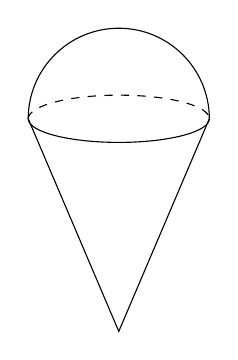
\begin{tikzpicture}
                \coordinate (O) at (0,0);
                \coordinate (V) at (0,-2.7);
                \draw (-1.15,0) arc[start angle=180,end angle=360,x radius=1.15,y radius=.3];
                \draw[dashed] (-1.15,0) arc[start angle=180,end angle=0,x radius=1.15,y radius=.3];
                \draw (-1.15,0) arc[start angle=180,end angle=0,x radius=1.15,y radius=1.15];
                \draw (-1.15,0)--(V)--(1.15,0);
            \end{tikzpicture}

            \textit{Hình 10.39}
        \end{center}
        \answerline
        \answerline

        \item Mái nhà hát Cao Văn Lầu và Trung tâm triển lãm Văn hoá Nghệ thuật tỉnh Bạc Liêu có hình dáng ba chiếc nón lá lớn nhất Việt Nam (H.10.40). Tính diện tích một mái nhà hình nón có đường kính bằng $45$ m và chiều cao bằng $24$ m (làm tròn kết quả đến hàng đơn vị của m$^2$).
        % TODO(HINH-NGUON): Hình 10.40 là ảnh thực tế công trình trong SGK trang 110; cần dùng asset/crop đúng từ nguồn, không redraw xấp xỉ bằng TikZ.
        \answerline
        \answerline
    \end{questions}
\end{exercises}

\section*{Ôn tập chương X}

\begin{practice}
    \subsection{Ôn tập chương X}

    \textbf{A. CÂU HỎI (Trắc nghiệm)}

    \begin{enumerate}
        \item Gọi $h$, $R$ lần lượt là độ dài của chiều cao và bán kính đáy của hình trụ. Diện tích xung quanh của hình trụ là
        \begin{tasks}(4)
            \task $S_{\mathrm{xq}}=2\pi Rh$.
            \task $S_{\mathrm{xq}}=\pi Rh$.
            \task $S_{\mathrm{xq}}=\pi Rl$.
            \task $S_{\mathrm{xq}}=\pi R^2h$.
        \end{tasks}
        \par\noindent\answerbox\par

        \item Một hình trụ có bán kính đáy bằng $6$ cm, chiều cao bằng $10$ cm. Thể tích của hình trụ này là
        \begin{tasks}(2)
            \task $V=300\pi$ (cm$^3$).
            \task $V=320\pi$ (cm$^3$).
            \task $V=340\pi$ (cm$^3$).
            \task $V=360\pi$ (cm$^3$).
        \end{tasks}
        \par\noindent\answerbox\par

        \item Một hình trụ có chu vi của đường tròn đáy bằng $4\pi a$, chiều cao bằng $a$. Thể tích của hình trụ này là
        \begin{tasks}(4)
            \task $V=2\pi a^3$.
            \task $V=4\pi a^3$.
            \task $V=16\pi a^3$.
            \task $V=\dfrac{4}{3}\pi a^3$.
        \end{tasks}
        \par\noindent\answerbox\par

        \item Hình trụ có bán kính đáy bằng $2\sqrt{3}$ cm và thể tích bằng $24\pi$ cm$^3$. Chiều cao của hình trụ này là
        \begin{tasks}(4)
            \task $h=2$ cm.
            \task $h=6$ cm.
            \task $h=2\sqrt{3}$ cm.
            \task $h=1$ cm.
        \end{tasks}
        \par\noindent\answerbox\par

        \item Gọi $l$, $h$, $R$ lần lượt là độ dài đường sinh, chiều cao và bán kính đáy của hình nón. Đẳng thức nào sau đây luôn đúng?
        \begin{tasks}(4)
            \task $l^2=h^2+R^2$.
            \task $\dfrac{1}{l^2}=\dfrac{1}{h^2}+\dfrac{1}{R^2}$.
            \task $R^2=h^2+l^2$.
            \task $l^2=hR$.
        \end{tasks}
        \par\noindent\answerbox\par

        \item Gọi $l$, $h$, $R$ lần lượt là độ dài đường sinh, chiều cao và bán kính đáy của hình nón. Diện tích xung quanh của hình nón là
        \begin{tasks}(4)
            \task $S_{\mathrm{xq}}=2\pi Rl$.
            \task $S_{\mathrm{xq}}=\pi Rh$.
            \task $S_{\mathrm{xq}}=\pi Rl$.
            \task $S_{\mathrm{xq}}=\pi R^2h$.
        \end{tasks}
        \par\noindent\answerbox\par

        \item Thể tích $V$ của hình nón có chiều cao bằng $a$ và độ dài đường sinh bằng $a\sqrt{5}$ là
        \begin{tasks}(4)
            \task $V=4\pi a^3$.
            \task $V=\dfrac{4}{3}\pi a^3$.
            \task $V=\dfrac{2}{3}\pi a^3$.
            \task $V=\dfrac{5}{3}\pi a^3$.
        \end{tasks}
        \par\noindent\answerbox\par

        \item Cho hình nón có diện tích xung quanh $25\pi$ cm$^2$, bán kính đường tròn đáy bằng $5$ cm. Độ dài đường sinh của hình nón là
        \begin{tasks}(4)
            \task $l=1$ cm.
            \task $l=\dfrac{5}{2}$ cm.
            \task $l=5$ cm.
            \task $l=3$ cm.
        \end{tasks}
        \par\noindent\answerbox\par

        \item Gọi $R$ là bán kính, $S$ là diện tích mặt cầu và $V$ là thể tích của hình cầu. Công thức nào sau đây là sai?
        \begin{tasks}(4)
            \task $3V=SR$.
            \task $S=4\pi R^2$.
            \task $V=\dfrac{4}{3}\pi R^3$.
            \task $S=\pi R^2$.
        \end{tasks}
        \par\noindent\answerbox\par

        \item Một mặt cầu có diện tích $36\pi$ m$^2$. Thể tích của hình cầu này là
        \begin{tasks}(4)
            \task $V=\dfrac{4}{3}\pi$ m$^3$.
            \task $V=36\pi$ m$^3$.
            \task $V=72\pi$ m$^3$.
            \task $V=108\pi$ m$^3$.
        \end{tasks}
        \par\noindent\answerbox\par
    \end{enumerate}

    \textbf{B. BÀI TẬP}

    \begin{questions}[resume=SBT]
        \item Một khối gỗ có dạng hình trụ, chiều cao bằng $50$ cm, đường kính đáy bằng $30$ cm.
        \begin{questions}
            \item Tính thể tích của khối gỗ.
            \item Nếu sơn phủ kín mặt bên ngoài khối gỗ thì diện tích cần sơn là bao nhiêu (làm tròn kết quả đến hàng đơn vị của cm$^2$)?
        \end{questions}
        \answerline
        \answerline

        \item Một chiếc nón lá có dạng một hình nón không có đáy, đường kính đáy bằng $80$ cm, chiều cao bằng $30$ cm. Tính diện tích mặt ngoài của chiếc nón (làm tròn kết quả đến hàng đơn vị của cm$^2$).
        \answerline
        \answerline

        \item Bạn Khôi có một chiếc bể cá làm bằng thuỷ tinh, có dạng hình cầu, đường kính $22$ cm. Khi nuôi cá, Khôi thường đổ vào bể lượng nước có thể tích bằng $\dfrac{2}{3}$ thể tích của bể. Tính thể tích nước bạn Khôi đổ vào bể khi nuôi cá (làm tròn kết quả đến hàng đơn vị của cm$^3$).

        \begin{center}
            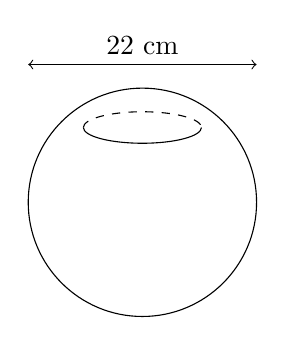
\begin{tikzpicture}
                \coordinate (O) at (0,0);
                \draw (O) circle[radius=1.45];
                \draw (-.75,.95) arc[start angle=180,end angle=360,x radius=.75,y radius=.20];
                \draw[dashed] (-.75,.95) arc[start angle=180,end angle=0,x radius=.75,y radius=.20];
                \draw[<->] (-1.45,1.75)--(1.45,1.75) node[midway,above] {$22$ cm};
            \end{tikzpicture}
        \end{center}
        \answerline
        \answerline

        \item Người ta cần làm một ống thoát nước hình trụ bằng bê tông (H.10.6) có chiều cao là $200$ cm, độ dày của thành ống là $15$ cm, đường kính của ống là $80$ cm. Tính lượng bê tông cần dùng để làm ống thoát nước nói trên.

        \begin{center}
            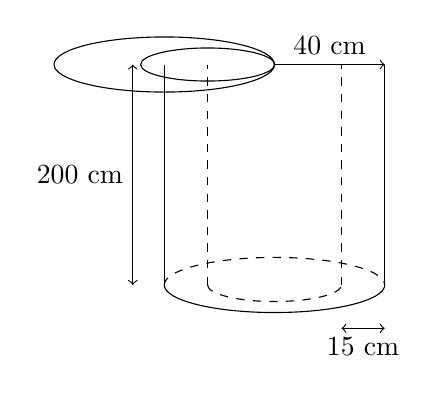
\begin{tikzpicture}
                \coordinate (O) at (0,2.8);
                \draw (-1.4,0) arc[start angle=180,end angle=360,x radius=1.4,y radius=.35];
                \draw[dashed] (-1.4,0) arc[start angle=180,end angle=0,x radius=1.4,y radius=.35];
                \draw (-1.4,0)--(-1.4,2.8) (1.4,0)--(1.4,2.8);
                \draw (-1.4,2.8) ellipse[x radius=1.4,y radius=.35];
                \draw (-.85,2.8) ellipse[x radius=.85,y radius=.21];
                \draw[dashed] (-.85,0) arc[start angle=180,end angle=360,x radius=.85,y radius=.21];
                \draw[dashed] (-.85,0)--(-.85,2.8) (.85,0)--(.85,2.8);
                \draw[<->] (-1.8,0)--(-1.8,2.8) node[midway,left] {$200$ cm};
                \draw[->] (0,2.8)--(1.4,2.8) node[midway,above] {$40$ cm};
                \draw[<->] (.85,-.55)--(1.4,-.55) node[midway,below] {$15$ cm};
            \end{tikzpicture}

            \textit{Hình 10.6}
        \end{center}
        \answerline
        \answerline

        \item Một hộp đựng bóng bàn có dạng hình trụ chứa vừa khít $3$ quả bóng bàn có cùng bán kính $R$ xếp theo chiều ngang (H.10.7).

        Gọi $S_1$ là tổng diện tích ba quả bóng bàn, $S_2$ là diện tích xung quanh của vỏ hộp hình trụ. Tính tỉ số $\dfrac{S_1}{S_2}$.

        \begin{center}
            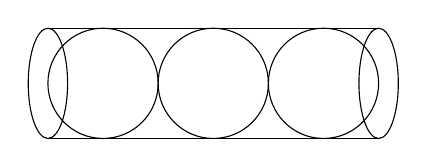
\begin{tikzpicture}
                \draw (-2.1,-.7)--(2.1,-.7) (-2.1,.7)--(2.1,.7);
                \draw (-2.1,0) ellipse[x radius=.25,y radius=.7];
                \draw (2.1,0) ellipse[x radius=.25,y radius=.7];
                \draw (-1.4,0) circle[radius=.7];
                \draw (0,0) circle[radius=.7];
                \draw (1.4,0) circle[radius=.7];
            \end{tikzpicture}

            \textit{Hình 10.7}
        \end{center}
        \answerline
        \answerline

        \item Một khối gỗ hình trụ tròn xoay có bán kính đáy bằng $1$ m, chiều cao bằng $2$ m. Người ta khoét từ hai đầu khối gỗ hai nửa hình cầu mà đường tròn đáy của khối gỗ là đường tròn lớn của mỗi nửa khối cầu (H.10.8). Tính tỉ số thể tích phần còn lại của khối gỗ và cả khối gỗ ban đầu.

        \begin{center}
            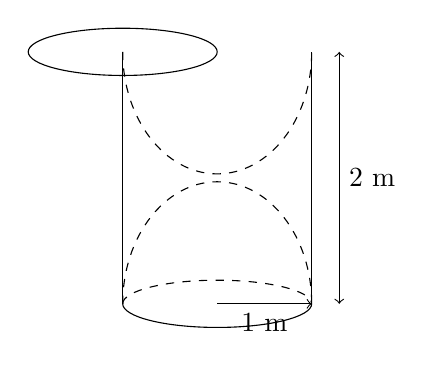
\begin{tikzpicture}
                \draw (-1.2,-1.6) arc[start angle=180,end angle=360,x radius=1.2,y radius=.3];
                \draw[dashed] (-1.2,-1.6) arc[start angle=180,end angle=0,x radius=1.2,y radius=.3];
                \draw (-1.2,-1.6)--(-1.2,1.6) (1.2,-1.6)--(1.2,1.6);
                \draw (-1.2,1.6) ellipse[x radius=1.2,y radius=.3];
                \draw[dashed] (-1.2,1.6) arc[start angle=180,end angle=360,x radius=1.2,y radius=1.55];
                \draw[dashed] (-1.2,-1.6) arc[start angle=180,end angle=0,x radius=1.2,y radius=1.55];
                \draw[<->] (1.55,-1.6)--(1.55,1.6) node[midway,right] {$2$ m};
                \coordinate (Obase) at (0,-1.6);
                \draw[->] (Obase)--(1.2,-1.6) node[midway,below] {$1$ m};
            \end{tikzpicture}

            \textit{Hình 10.8}
        \end{center}
        \answerline
        \answerline

        \item Một dụng cụ gồm một phần có dạng hình trụ và một phần có dạng hình nón với kích thước như Hình 10.9.

        \begin{center}
            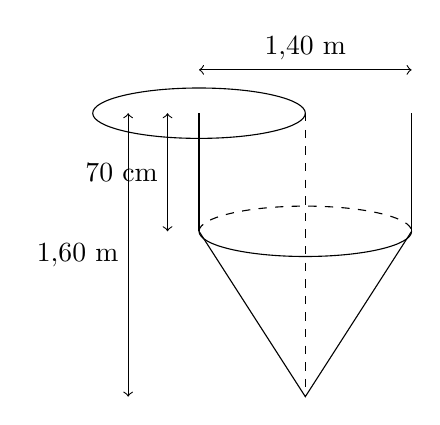
\begin{tikzpicture}
                \coordinate (Otop) at (0,1.5);
                \coordinate (Omix) at (0,0);
                \coordinate (V) at (0,-2.1);
                \draw (-1.35,0)--(-1.35,1.5) (1.35,0)--(1.35,1.5);
                \draw (-1.35,1.5) ellipse[x radius=1.35,y radius=.32];
                \draw (-1.35,0) arc[start angle=180,end angle=360,x radius=1.35,y radius=.32];
                \draw[dashed] (-1.35,0) arc[start angle=180,end angle=0,x radius=1.35,y radius=.32];
                \draw (-1.35,0)--(V)--(1.35,0);
                \draw[dashed] (Otop)--(V);
                \draw[<->] (-1.35,2.05)--(1.35,2.05) node[midway,above] {$1{,}40$ m};
                \draw[<->] (-1.75,0)--(-1.75,1.5) node[midway,left] {$70$ cm};
                \draw[<->] (-2.25,-2.1)--(-2.25,1.5) node[midway,left] {$1{,}60$ m};
            \end{tikzpicture}

            \textit{Hình 10.9}
        \end{center}

        \begin{questions}
            \item Tính thể tích của dụng cụ này.
            \item Tính diện tích mặt ngoài của dụng cụ (không tính nắp đáy, kết quả làm tròn đến hàng phần mười của m$^2$).
        \end{questions}
        \answerline
        \answerline
        \answerline
    \end{questions}
\end{practice}
